%!TEX root = ../../super_main.tex

\chapter{Quality Assurance}
\label{cha:quality_assurance}

This section describes the different measures we have used in order ensure the quality of our developed product 
\todo{Write more intro to QA}. 
\\\\
When we executed tests that required that we run the code om some device, we always attempted to run it on multiple different devices in order to support several different hardware configurations and also that we are compatible with multiple Android versions. The phones we have available all run stock Android versions from the Android open source project. This might indicate that we also cover additional OS versions that are based on the stock versions, since if we find some bug when we test against the stock version, it is most likely also present in the modified version. 


\todo{Overvej at lave pair programming section}

\section{Automated Unit Test}
\label{sec:automated_unit_test}

\todo[inline]{Write about automated unit tests}

\section{Continuous Integration}
\label{sec:continuous_integration}
As mentioned in \secref{sec:extreme_programming}, we wanted a continuous integration server in order to ensure that our code base always was at a stable state. We installed Jenkins on the same server that makes up the server part of our client-server architecture because it was easily available. Jenkins is an open source automation server, which supports various different plugins that helps with builds, viewing test results, etc. We configured this Jenkins server to be notified whenever our Github version control code repositories for both Android and PHP code were changed. When this notification happened, Jenkins would build the corresponding project and run its tests. Whenever the build projects would go from a previously successful build to a now failing build or vice versa, the Jenkins system would send out mails to our group, so we were aware that something went wrong or that it was now fixed again. This made it possible for us to give immediate attention to issues that we did not catch before pushing our content to the version control. See \figref{fig:jenkins_front_page} for an illustration of how the front page of Jenkins. In the left side, the build queue can be seen, which shows if any builds are currently running. In the center, the various projects that are currently configured for the Jenkins setup can be seen. The blue circle changes to red if the most recent build was a failure, and besides that, it can be seen how long time has passed since the most recent pass, most recent failure, and how long the last build took to finish. By clicking on one of the projects, statistics can be seen for checkstyes errors, code coverage, and test results. 

\begin{figure}[!htbp]
    \centering
    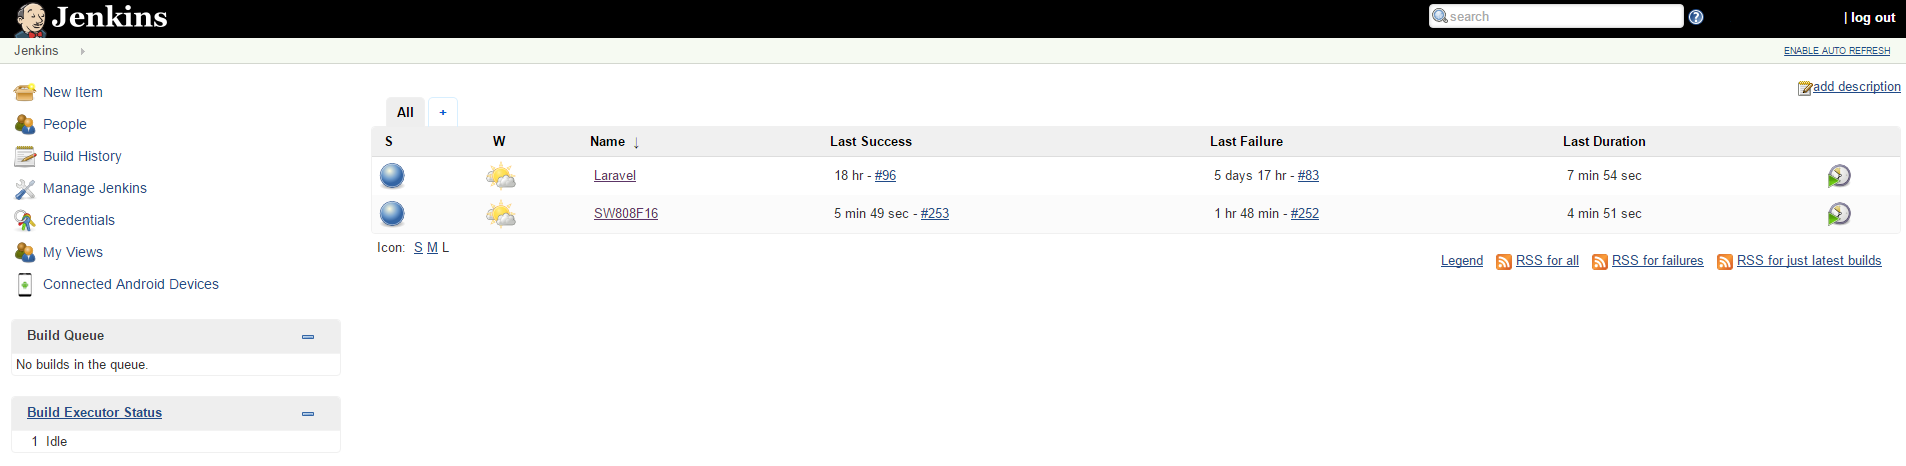
\includegraphics[width=\textwidth]{graphic/quality_assurance/jenkins_frontpage.png}
    \caption{Jenkins CI front page}
    \label{fig:jenkins_front_page}
\end{figure}
\FloatBarrier

We used this extensively during the development, because when several people merge their work into the master branch of the version control several times per day, something is bound to go wrong eventually. This ensured that we always knew if something was wrong with either of our projects, so we knew when we needed to allocate people for fixing it. 

\section{Monkey Test}
\label{sec:monkey_test}
We executed UI/Application Exerciser Monkey tests on the android code. The exerciser monkey generates pseudo-random streams of user events, which can be used to test the robustness of the application. The monkey is able to stress-test the application because of frequent button clicks, etc., such that it most likely crashes if there are memory leaks or other bad implementations. It furthermore provides the possibility of simulating irradical user behavior, that might perform some trace of actions that human users would not typically follow, which might crash the application. 
\\\\
We started by running one trace on 50000 inputs on a Galaxy Nexus phone, where the application crashed after 46000 actions, which allowed us to take a look at the exception and resolve it. Afterwards the monkey ran for 2 hours straight without crashing, and we therefore think the application is rather robust.
\\\\
Following this we also ran the monkey for a while on a Nexus 5 device which had Android 6.x, in contrast to the 5.x on the Galaxy Nexus. Here it also seemed to run without any difficulties, which gives some indication that our application is resilient in terms of different configurations and also compatible with different versions of Android without issues.

\section{Pair Group Review}
\label{sec:pair_group_review}

Two times during the project period we arranged meetings with another software student group at Aalborg University, where we presented the current states of our projects and provided critique for each other. 
\\\\
\todo[inline]{Write what we achieved from the pair group reviews}